\documentclass[10pt,twocolumn]{ctexart}
\usepackage[margin=0.72in]{geometry}
\usepackage{graphicx}
\usepackage{booktabs}
\usepackage{amsmath}
\usepackage{amssymb}
\usepackage{hyperref}
\usepackage{xcolor}
\usepackage{listings}
\usepackage{caption}
\captionsetup{font=small,labelfont=bf}
\lstset{
  basicstyle=\ttfamily\footnotesize,
  breaklines=true,
  frame=single,
  columns=fullflexible
}
\hypersetup{colorlinks=true,linkcolor=blue,urlcolor=blue,citecolor=blue}

\setCJKmainfont{SimSun}[AutoFakeBold=2.5]
\setCJKsansfont{Microsoft YaHei}[AutoFakeBold=2.5]
\setCJKmonofont{Microsoft YaHei}

\title{\vspace{-1.2em}基于验证技能接口与执行反馈的LLM辅助移动机器人任务规划}
\author{候选人\small 面试作业}
\date{\vspace{-0.8em}}

\begin{document}
\maketitle

\begin{abstract}
本文介绍一个将自然语言指令转换为少量、经过验证的高层机器人技能调用的单机器人系统。
系统运行于 ROS~2 Humble 与 Webots~R2025a，部署在 Windows 主机上的 WSL2 中。
任务级规划器只能从固定的三项技能白名单中选择；多层验证器在每个调用执行前进行检查；
有界恢复模块观察每个结构化执行结果，并在重试、避障恢复、带执行反馈的一次性 LLM 重规划、
安全停止上报之间做出决策。实验表明：系统能以 0.049\,m 的位置误差到达目标，
能可靠执行多航点任务，能安全拒绝越界与未知技能计划，并能给出“LLM 收到超时反馈后重新生成计划”的闭环执行轨迹。
\end{abstract}

\section{引言}
\label{sec:intro}
大语言模型可以将自然语言翻译为结构化工具调用，但直接在机器人上执行其输出并不安全。
本作业要求：LLM 只能\textbf{选择}已有的高层技能，不得直接发布速度指令，也不得执行生成的代码。
本文的设计目标是可靠性、显式技能契约、严格验证与可复现实验。

系统遵循如下闭环：\texttt{Plan} $\rightarrow$ \texttt{Validate} $\rightarrow$
\texttt{Execute} $\rightarrow$ \texttt{Observe} $\rightarrow$ \texttt{Recover}。
主要贡献包括：
\begin{itemize}
  \item 具有固定白名单与 JSON Schema 契约的验证式技能接口；
  \item \texttt{navigate\_to}、\texttt{follow\_waypoints}、\texttt{stop} 三个技能的 ROS~2 实现；
  \item 集中管理规划、验证、执行、观察与恢复的闭环任务代理 \texttt{TaskAgent}；
  \item 规则规划器与可消费结构化执行反馈进行有界重规划的 OpenAI 兼容 LLM 规划器；
  \item 针对越界地点、未知技能、超时与障碍阻塞的有界恢复；
  \item 可复现的 WSL2/Webots 环境与 JSONL 执行日志。
\end{itemize}

\section{系统架构}
\label{sec:arch}
图~\ref{fig:arch} 给出系统架构。规划器生成原始计划（\texttt{SkillCall[]}）；
验证器在机器人执行任何动作之前检查计划；只有通过验证的调用才会到达技能执行器；
执行器调用 \texttt{RobotSkills} ROS~2 节点；该节点发布速度指令，并从 Webots 读取位置、航向与激光反馈。
每个技能返回结构化 \texttt{SkillResult}；执行失败时，恢复模块决定重试、后退重试、
带 \texttt{ExecutionFeedback} 的重规划、或停止上报。所有事件追加写入 JSONL 日志。

\begin{figure}[t]
  \centering
  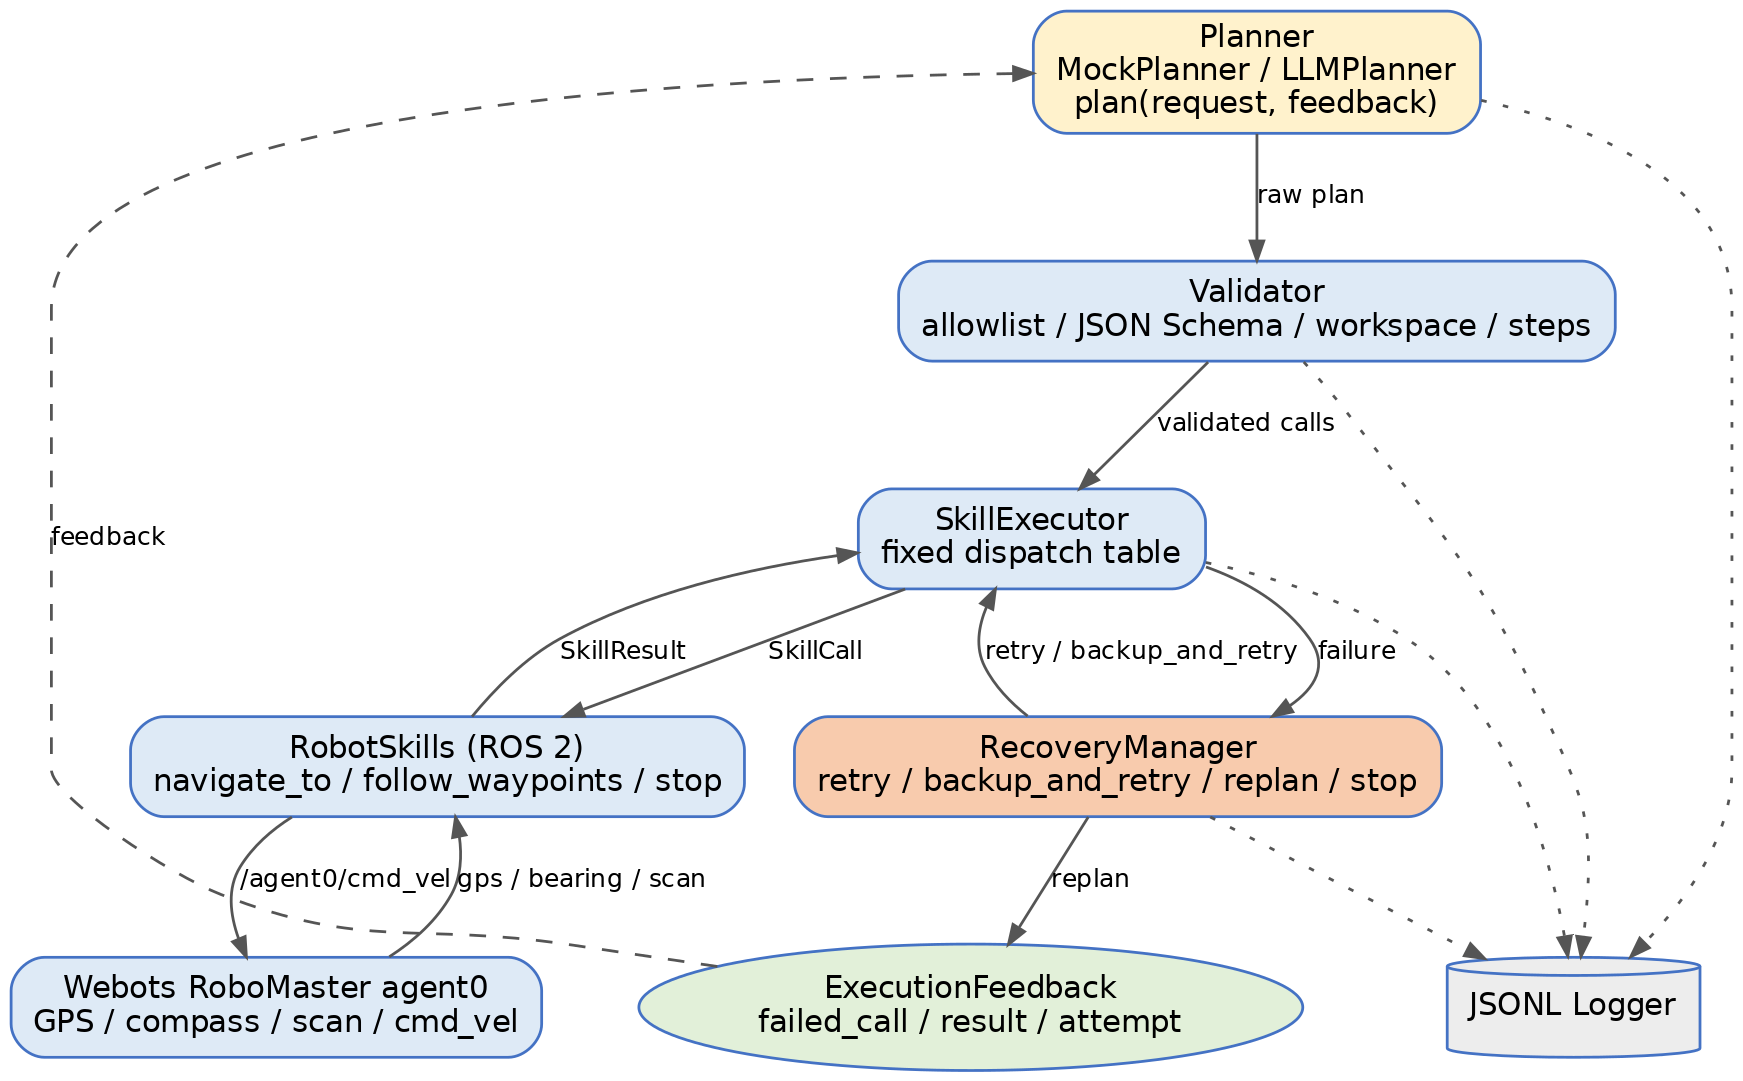
\includegraphics[width=\linewidth]{figures/architecture_feedback.png}
  \caption{闭环系统架构。虚线为 LLM 规划器用于有界重规划的执行反馈通道。}
  \label{fig:arch}
\end{figure}

\subsection{模块划分}
仓库将任务级代理与 ROS~2 技能层分离：
\begin{itemize}
  \item \texttt{agent/task\_agent.py}：负责 Plan--Validate--Execute--Observe--Recover 闭环；
  \item \texttt{agent/planner.py}：规则规划器与可选 LLM 规划器；
  \item \texttt{agent/registry.py}：机器可读技能注册表；
  \item \texttt{agent/validator.py}：六层验证；
  \item \texttt{agent/executor.py}：到三项技能的固定分发表；
  \item \texttt{agent/recovery.py}：有界恢复决策；
  \item \texttt{agent/models.py}：\texttt{SkillCall}、\texttt{SkillResult}、\texttt{ValidationResult}、\texttt{ExecutionFeedback}；
  \item \texttt{agent/logger.py}：JSONL 事件日志；
  \item \texttt{robot\_skills/skills.py}：技能的 ROS~2 实现。
\end{itemize}

\subsection{技能接口}
表~\ref{tab:skills} 概括三项技能。注册表是唯一事实来源：同一份定义既生成验证器使用的
JSON Schema，也生成暴露给 LLM 的工具列表。

\begin{table}[t]
\centering
\caption{技能接口摘要。}
\label{tab:skills}
\small
\begin{tabular}{p{0.20\linewidth}p{0.70\linewidth}}
\toprule
技能 & 契约 \\
\midrule
\texttt{navigate\_to} &
参数：$x,y,\theta$；成功条件：位置误差 $\le 0.05$\,m 且航向误差 $\le 0.10$\,rad；超时：30\,s \\
\texttt{follow\_waypoints} &
参数：航点列表；失败时返回最后到达的航点下标；超时：每个航点 30\,s \\
\texttt{stop} &
发布零速度；成功条件：已发布零速度；超时：2\,s \\
\bottomrule
\end{tabular}
\end{table}

\section{实现细节}
\label{sec:impl}

\subsection{ROS~2 技能层}
\texttt{RobotSkills} 节点订阅 \texttt{/agent0/gps}（\texttt{PointStamped}）获取位置，
订阅 \texttt{/agent0/compass/bearing}（\texttt{FloatStamped}）获取航向，
并在 \texttt{/agent0/cmd\_vel} 上发布 \texttt{Twist} 速度指令。
Webots 罗盘方位角以顺时针为正，而 ROS 偏航角以逆时针为正，因此节点按如下公式转换：
\begin{equation}
  \psi = \mathrm{normalize}(-\mathrm{radians}(\mathrm{bearing})).
\end{equation}

\subsection{全向 \texttt{navigate\_to}（PID）}
RoboMaster 底盘为全向底盘。控制器无需先旋转再直行，而是直接在车体系中平移，
仅在最后对航向进行原地旋转校正：
\begin{align}
  e_x &= x_d - x, \qquad e_y = y_d - y, \\
  v_x^{w} &= \mathrm{clamp}\big(k_p e_x + k_i \textstyle\int e_x dt + k_d \tfrac{d e_x}{dt}, -v_{\max}, v_{\max}\big), \\
  v_y^{w} &= \mathrm{clamp}\big(k_p e_y + k_i \textstyle\int e_y dt + k_d \tfrac{d e_y}{dt}, -v_{\max}, v_{\max}\big), \\
  v_x^{b} &= \cos\psi\, v_x^{w} + \sin\psi\, v_y^{w}, \\
  v_y^{b} &= -\sin\psi\, v_x^{w} + \cos\psi\, v_y^{w}.
\end{align}
当位置误差大于容差时，节点发布 $(v_x^{b}, v_y^{b}, 0)$；否则发布 $(0,0,\omega)$，
其中 $\omega = \mathrm{clamp}\big(k_p^\theta e_\theta + k_i^\theta \textstyle\int e_\theta dt + k_d^\theta \tfrac{d e_\theta}{dt}, -\omega_{\max}, \omega_{\max}\big)$。
成功条件为
\begin{equation}
  \sqrt{e_x^2+e_y^2} \le 0.05\,\mathrm{m}
  \quad\text{且}\quad |e_\theta| \le 0.10\,\mathrm{rad}.
\end{equation}
超时后节点停止机器人并返回 \texttt{success=false, reason="timeout"}。

\subsection{\texttt{follow\_waypoints} 与 \texttt{stop}}
\texttt{follow\_waypoints} 依次调用 \texttt{navigate\_to} 并维护
\texttt{last\_reached\_index}。若某个航点失败，节点停车并返回该下标。
\texttt{stop} 发布零速度并返回结构化结果。

\subsection{障碍安全层}
\texttt{navigate\_to} 同时订阅 \texttt{/scan}。在发布平移指令前，它检查意图运动方向
30 度锥角内的最小有效距离。若该距离不超过 0.35\,m，技能停车并返回
\texttt{success=false, reason="obstacle\_blocked"}。任务级恢复随后执行后退、旋转并重试一次。

\subsection{闭环任务代理}
\texttt{TaskAgent} 拥有完整执行循环。它首先请求规划器生成计划并记录原始计划；
验证器在运动前检查计划，无效则拒绝。对每个通过验证的调用，执行器调用对应技能并记录观察到的
\texttt{SkillResult}。成功的调用被记录并继续执行。失败时，\texttt{RecoveryManager} 选择有界动作：
\begin{itemize}
  \item \texttt{retry}：超时后重新执行同一调用一次；
  \item \texttt{backup\_and\_retry}：障碍阻塞后后退、旋转并重试一次；
  \item \texttt{replan}：将 \texttt{ExecutionFeedback} 发送给 LLM 规划器并请求新计划
        （仅当规划器支持反馈且重规划预算未耗尽）；
  \item \texttt{stop\_and\_report}：停车并返回失败。
\end{itemize}
重规划产生的新计划必须在任何机器人动作前重新通过验证。若规划器返回相同计划，代理安全停止而不会循环。
重规划次数由 \texttt{--max-replans} 限定（默认 1）。

\subsection{验证层}
验证器共六层：计划长度、固定白名单、JSON Schema、工作空间边界、前置条件、重试/重规划次数限制。
允许的工作空间为 $x,y \in [-1.5,1.5]$\,m。表~\ref{tab:validation} 列出各层及对应失败原因。

\begin{table}[t]
\centering
\caption{验证层及产生的失败原因。}
\label{tab:validation}
\small
\begin{tabular}{p{0.38\linewidth}p{0.54\linewidth}}
\toprule
验证层 & 失败原因 \\
\midrule
计划长度 & \texttt{too\_many\_steps} \\
白名单 & \texttt{unknown\_skill} \\
JSON Schema & \texttt{schema\_invalid} \\
工作空间边界 & \texttt{target\_out\_of\_workspace} \\
前置条件 & \texttt{precondition\_failed} \\
重试/重规划限制 & \texttt{stop\_and\_report} \\
\bottomrule
\end{tabular}
\end{table}

\section{实验与结果}
\label{sec:exp}

\subsection{实验平台}
实验平台为 Windows~11 + WSL2 Ubuntu~22.04 + ROS~2 Humble + Webots~R2025a。
GPU 为 AMD Radeon RX~9070~XT（16\,GB）。WSLg 提供基于 Mesa D3D12 驱动的硬件加速
OpenGL~4.2 上下文：\texttt{glxinfo} 报告渲染器
\texttt{D3D12 (AMD Radeon RX 9070 XT)} 且 \texttt{Accelerated: yes}；
\texttt{glxgears} 约 140\,FPS。

\subsection{任务级回归测试}
表~\ref{tab:results} 给出闭环重构后的完整回归结果。成功用例以 0.0494\,m 的位置误差到达
storage。多航点用例到达全部航点并报告 \texttt{last\_reached\_index=1}。
越界地点在 mock 规划器下被工作空间层拒绝；真实 LLM 对越界请求返回空工具列表，
验证器在执行前拒绝。未知技能被白名单层拒绝。强制超时用例重试一次后被安全停止并上报。
障碍恢复用例在后退+旋转重试后成功；持续障碍用例则停车并上报目标被阻塞。
真实云 LLM 规划器使用 OpenAI 兼容端点与 gpt-5.5 模型，正确生成了
\texttt{navigate\_to} 以及 \texttt{follow\_waypoints + stop} 计划。

关键新结果是 R12。LLM 首先规划前往 charging\_station。在连续两次超时观测之后，
恢复层将结构化 \texttt{ExecutionFeedback} 发回 LLM。LLM 返回新的经过验证的计划，
改为前往 storage；由于超时仍被强制为 1 秒，该计划最终被安全停止并上报。
因此 JSONL 日志包含完整序列：
\texttt{raw\_plan} $\rightarrow$ \texttt{skill\_result} $\rightarrow$
\texttt{recovery\_decision} $\rightarrow$ \texttt{feedback\_to\_planner}
$\rightarrow$ \texttt{replanned\_plan} $\rightarrow$ \texttt{validation}
$\rightarrow$ \texttt{skill\_result} $\rightarrow$ \texttt{final\_outcome}。

\begin{table*}[t]
\centering
\caption{闭环代理的任务级回归结果。}
\label{tab:results}
\small
\begin{tabular}{llcccl}
\toprule
ID & 指令 & 规划器/模式 & 结果 & 技能调用 & 恢复动作 \\
\midrule
R1 & Go to storage. & mock / direct & 成功，18.58\,s，0.0494\,m & 1 & 无 \\
R2 & Visit storage, then workbench, and stop. & mock / direct & 成功，38.27\,s & 2 & 无 \\
R3 & Go to storage. & mock / map (A*) & 成功，17.73\,s，\texttt{map\_reached} & 1 & 无 \\
R4 & Go to space\_station. & mock & 拒绝 & 0 & 中止，\texttt{target\_out\_of\_workspace} \\
R5 & Go to entrance and fly. & mock & 拒绝 & 0 & 中止，\texttt{unknown\_skill} \\
R6 & Go to charging\_station，强制 1\,s 超时 & mock / direct & 失败 & 2 & 重试一次后停止上报 \\
R7 & Go to storage，障碍后消失 & mock / direct & 成功，0.0500\,m & 2 & 后退、旋转、重试一次 \\
R8 & Go to storage，障碍持续存在 & mock / direct & 失败 & 2 & 后退、旋转、停止上报 \\
R9 & Go to storage. & 真实 LLM / direct & 成功，16.43\,s，0.0499\,m & 1 & 无 \\
R10 & Visit storage, then workbench, and stop. & 真实 LLM / direct & 成功，38.70\,s & 2 & 无 \\
R11 & Go to space\_station. & 真实 LLM & 拒绝 & 0 & LLM 返回空计划，中止 \\
R12 & Go to charging\_station，强制 1\,s 超时 & 真实 LLM / direct & 失败 & 4 & 重试，\textbf{带反馈重规划}，重试，停止 \\
\bottomrule
\end{tabular}
\end{table*}

\subsection{手动控制与标定}
表~\ref{tab:calib} 给出参考 \texttt{wheels\_controller} 的观测响应。该控制器使用了错误的
轮半径常量（0.26，而 URDF 中为 0.06），因此技能层采用闭环反馈而非开环定时。

\begin{table}[t]
\centering
\caption{观测到的指令响应。}
\label{tab:calib}
\small
\begin{tabular}{lcc}
\toprule
指令 & 观测运动 & 近似响应 \\
\midrule
\texttt{linear.x = 1.0} & 2\,s 内移动 0.20\,m & 0.10\,m/s \\
\texttt{linear.y = 1.0} & 2\,s 内移动 0.22\,m & 0.11\,m/s \\
\texttt{angular.z = 5.0} & 2\,s 内转动 127$^\circ$ & 1.11\,rad/s \\
\bottomrule
\end{tabular}
\end{table}

\section{讨论}
\label{sec:discussion}

\subsection{安全性}
LLM 从不获得直接执行器权限。它只能从三项白名单技能中选择，且每个提议调用在执行前都经过验证器。
执行器将技能名映射到具有预定义签名的 Python 方法；任何生成的 Python、Shell 或 ROS 命令都不会被执行。
越界目标、未知技能、参数错误、步数超限与空计划均被拒绝。超时或障碍阻塞最终都会以零速度指令
和结构化失败报告结束。

\subsection{执行反馈}
重构后的代理使执行反馈显式且有界。LLM 只看到任务级信息：原始请求、失败调用、
结构化结果、恢复消息与已完成工作；它从不接触原始传感器数据。反馈路径由规则触发，
因此系统在使用 mock 规划器时保持确定性和可测试性，同时支持真实 LLM 对比实验。

\subsection{可复现性}
系统可依据仓库与 \texttt{docs/environment.md} 中的环境说明复现。所需依赖包括 ROS~2 Humble、
Webots~R2025a、\texttt{webots\_ros2} 2025.0.0 与参考包 \texttt{webots\_ros2\_robomaster}
的世界资源。Webots 资源缓存与参考 \texttt{protos/meshes} 目录已在文档中说明。
生成的 JSONL 日志作为示例提交。

\subsection{局限性}
最终配置在 WSL2 中通过 WSLg 运行 Webots。WSLg 存在一定的 D3D12 转换与 Xwayland 合成开销，
流畅度不如可选的 Windows 原生 Webots 模式，但足以完成本作业。参考环境没有
\texttt{/agent0/odom} 话题，因此技能层使用 \texttt{/agent0/gps} 获取位置、
\texttt{/agent0/compass/bearing} 获取航向。参考 \texttt{wheels\_controller} 的轮半径常量有误，
因此必须采用闭环控制。当前 LLM 重规划为一次性、规则触发，尚未对原始计划与重规划计划进行
除“完全相同检测”之外的更深比较。

\subsection{后续工作}
未来工作包括：让 LLM 规划器基于完整执行轨迹与显式失败语义进行推理；使用 \texttt{/scan}
进行动态避障；增加专用里程计话题；以及 Docker/WSL 一键化环境。

\section{结论}
\label{sec:conclusion}
本文介绍了一个可靠、经过验证的 LLM 辅助任务规划系统。系统将规划、验证、执行、观察与恢复分离；
强制固定白名单；每个技能返回结构化结果；并通过有界执行反馈将执行结果送回 LLM 规划器。
实验证明了位姿到达、多航点执行、基于地图的 A* 导航、越界与未知技能拒绝、障碍恢复，
以及真实 LLM 在观测到超时后进行重规划的完整闭环轨迹。

\begin{thebibliography}{9}
\bibitem{ros2}
ROS~2 Humble 文档。\url{https://docs.ros.org/en/humble/}
\bibitem{webots}
Cyberbotics Webots。\url{https://cyberbotics.com/}
\bibitem{webotsros2}
\texttt{webots\_ros2}。\url{https://github.com/cyberbotics/webots_ros2}
\bibitem{robomaster}
\texttt{webots\_ros2\_robomaster}。
\url{https://github.com/MohismLab/webots_ros2_robomaster}
\bibitem{wslg}
Microsoft WSLg。\url{https://github.com/microsoft/wslg}
\bibitem{mesa}
Mesa D3D12 驱动。\url{https://docs.mesa3d.org/drivers/d3d12.html}
\bibitem{openai}
OpenAI 兼容函数调用。
\url{https://platform.openai.com/docs/guides/function-calling}
\end{thebibliography}

\end{document}
